\documentclass[../main]{subfiles}
\ifSubfilesClassLoaded{\setcounter{chapter}{0}}{}
\begin{document}

\chapter{Pendahuluan dan Orientasi Buku}

\section{Tujuan Buku Ajar}

Buku ajar ini dirancang sebagai panduan komprehensif untuk menguasai \crypt{Kriptografi} dalam konteks Programme Studi Matematika S1 \cite{stinson2018}. Fokus utama buku ini adalah pada pemahaman matematis, konsep teoretis, dan implementasi algoritma kriptografi menggunakan bahasa pemrograman C. Tujuan spesifik buku ini adalah:

\begin{enumerate}
  \item Memberikan pemahaman mendalam tentang prinsip-prinsip dasar kriptografi dan keamanan informasi
  \item Mengembangkan kemampuan menerapkan matematika (aritmetika modular, teori bilangan) dalam konteks kriptografi
  \item Membangun keterampilan implementasi algoritma kriptografi klasik dan modern dalam bahasa C
  \item Menumbuhkan kemampuan analisis kriptanalisis terhadap cipher sederhana
  \item Memfasilitasi pencapaian CPL dan CPMK yang telah ditetapkan dalam RPS berbasis OBE
\end{enumerate}

Setelah mempelajari buku ini secara menyeluruh, mahasiswa diharapkan mampu:
\begin{itemize}
  \item Menjelaskan konsep dasar kriptografi (confidentiality, integrity, authenticity)
  \item Menerapkan aritmetika modular dan algoritma Euclid dalam konteks kriptografi
  \item Mengimplementasikan cipher Caesar, Vigenère, dan RSA dalam bahasa C
  \item Menganalisis kelemahan cipher klasik melalui frequency analysis dan Kasiski examination
  \item Merancang dan menganalisis protokol kriptografi dasar
\end{itemize}

Pendidikan kriptografi modern membutuhkan fondasi matematis yang kuat termasuk teori bilangan, aljabar linear, dan matematika diskrit untuk memahami algoritma enkripsi yang kompleks. Menurut Coursera, pemahaman tentang modular arithmetic, algoritma Euclid, dan teorema sisa China merupakan prasyarat esensial untuk menguasai kriptografi tingkat lanjut. Kurikulum yang dirancang dengan baik mengintegrasikan konsep matematika murni dengan aplikasi praktis dalam keamanan digital, mempersiapkan mahasiswa untuk karir di bidang keamanan siber.

Profesi kriptografer menuntut kombinasi unik antara keahlian matematika, pemrograman, dan pemahaman keamanan siber untuk mengembangkan cipher baru dan melindungi data sensitif. Industri saat ini sangat membutuhkan ahli kriptografi yang mampu membuat solusi keamanan inovatif seiring dengan evolusi ancaman digital yang terus berubah. Mahasiswa yang menguasai materi dalam buku ini akan memiliki kompetensi untuk berkarir di lembaga pemerintah, institusi keuangan, atau perusahaan teknologi yang memprioritaskan keamanan data.

\section{Keterkaitan Buku Ajar dan RPS OBE}

Buku ajar ini dirancang dengan ketat mengikuti Rencana Pembelajaran Semester (RPS) Mata Kuliah Kriptografi yang berbasis \textbf{Outcome-Based Education (OBE)}. Setiap bab dipetakan secara eksplisit ke Capaian Pembelajaran Mata Kuliah (CPMK) dan Sub-CPMK yang tercantum dalam silabus.

Outcome-Based Education (OBE) merupakan pendekatan kurikulum yang berfokus pada hasil pembelajaran (learning outcomes) yang harus dicapai mahasiswa, bukan sekadar materi yang diajarkan oleh dosen. Menurut Wikipedia, OBE mengorganisir seluruh sistem pendidikan menuju apa yang dianggap esensial bagi pembelajar untuk berhasil dilakukan di akhir pengalaman belajar mereka. Pendekatan ini memberikan kejelasan tentang harapan pencapaian dan fleksibilitas dalam metode instruksional, memungkinkan dosen untuk menggunakan berbagai teknik pengajaran dan asesmen yang sesuai dengan kebutuhan mahasiswa.

Implementasi OBE dalam kriptografi memastikan setiap kompetensi yang dipelajari dapat diukur dan diverifikasi melalui asesmen yang terstruktur. Model pembelajaran berbasis outcome ini memungkinkan perbandingan standar kompetensi antar institusi dan memfasilitasi transisi mahasiswa ke dunia kerja dengan bukti pencapaian kompetensi yang jelas. Mahasiswa menjadi lebih terlibat dan bertanggung jawab atas pembelajaran mereka sementara dosen berperan sebagai fasilitator yang mengarahkan pencapaian kompetensi yang telah ditetapkan.

\begin{table}[htbp]
\centering
\small
\begin{tabular}{|c|c|p{7cm}|}
\hline
\textbf{Bab} & \textbf{Sub-CPMK} & \textbf{Materi Terkait} \\
\hline
I & -- & Orientasi dan panduan belajar \\
\hline
II & 1.1, 1.2, 1.3 & Landasan teori, model keamanan, simetris vs asimetris \\
\hline
III & 2.1, 2.2 & Matematika kriptografi, Euclid, fast exponentiation \\
\hline
IV & 3.1, 3.2 & Caesar, Vigenère, substitusi, implementasi C \\
\hline
V & 4.1 & DES, AES, mode operasi block cipher \\
\hline
VI & 4.2 & RSA, implementasi C \\
\hline
VII & 5.1, 5.2 & Fungsi hash, tanda tangan digital \\
\hline
VIII & 6.1 & Protokol Diffie-Hellman, manajemen kunci \\
\hline
IX & 7.1 & Kriptanalisis, frequency analysis, Kasiski \\
\hline
X & 8.1, semua & Evaluasi, refleksi, integrasi kompetensi \\
\hline
\end{tabular}
\caption{Petakan Bab ke Sub-CPMK}
\end{table}

Pendekatan OBE menekankan bahwa setiap aktivitas pembelajaran---materi, latihan, praktikum, dan asesmen---harus diarahkan untuk mencapai kompetensi yang terukur. Dengan demikian, mahasiswa dapat memantau kemajuan mereka secara mandiri melalui checklist pencapaian yang disediakan di setiap bab.

\section{Cara Menggunakan Buku Ajar}

Pembelajaran disarankan dilakukan secara berurutan dari Bab I hingga Bab X (dan bab tambahan jika tersedia), karena setiap konsep dibangun di atas materi sebelumnya. Bab II menjadi fondasi teoretis, Bab III memperkuat matematika kriptografi, dan bab-bab berikutnya berfokus pada implementasi serta analisis keamanan yang lebih kompleks.

\subsection{Alur Pembelajaran yang Kohesif}

Setiap bab dirancang untuk menjadi landasan bagi bab berikutnya:
\begin{itemize}
  \item \textbf{Bab II} memberikan \textit{big picture} keamanan informasi yang menjawab "mengapa kita perlu kriptografi?"
  \item \textbf{Bab III} menjawab "bagaimana matematika membuat kriptografi mungkin?" dengan fondasi yang akan digunakan langsung di Bab IV
  \item \textbf{Bab IV} menerapkan matematika Bab III dalam cipher klasik, mempersiapkan Anda untuk algoritma modern di Bab V
  \item \textbf{Bab V-VII} membangun dari cipher klasik ke algoritma modern, dengan matematika yang semakin kompleks
  \item \textbf{Bab VIII-IX} mengintegrasikan semua konsep dalam protokol dan analisis keamanan nyata
\end{itemize}

\subsection{Struktur OBE untuk Pembelajaran Terukur}

Gunakan struktur OBE di setiap bab sebagai panduan belajar. Komponen utama yang perlu diikuti adalah:
\begin{itemize}
  \item \textbf{Sub-CPMK}: target kompetensi yang harus dicapai
  \item \textbf{Materi Pokok}: teori, contoh numerik, dan kode C
  \item \textbf{Aktivitas Pembelajaran}: praktikum, diskusi, atau studi kasus
  \item \textbf{Latihan}: penguatan konsep sebelum asesmen
  \item \textbf{Asesmen}: alat ukur pencapaian Sub-CPMK
  \item \textbf{Checklist}: evaluasi diri setelah belajar
\end{itemize}

\subsection{Koneksi Teori dan Praktik}

Setiap bab dirancang dengan keseimbangan antara:
\begin{itemize}
  \item \textbf{Teori}: Konsep matematis dan prinsip kriptografi
  \item \textbf{Implementasi}: Kode C yang menunjukkan bagaimana teori bekerja dalam praktik
  \item \textbf{Analisis}: Mengapa suatu desain aman atau tidak
\end{itemize}

Agar pembelajaran konsisten, alokasikan waktu belajar secara proporsional antara membaca materi, praktik, latihan, dan refleksi. Grafik berikut bersifat ilustratif dan dapat disesuaikan dengan kebutuhan belajar masing-masing mahasiswa.

\begin{figure}[htbp]
  \centering
  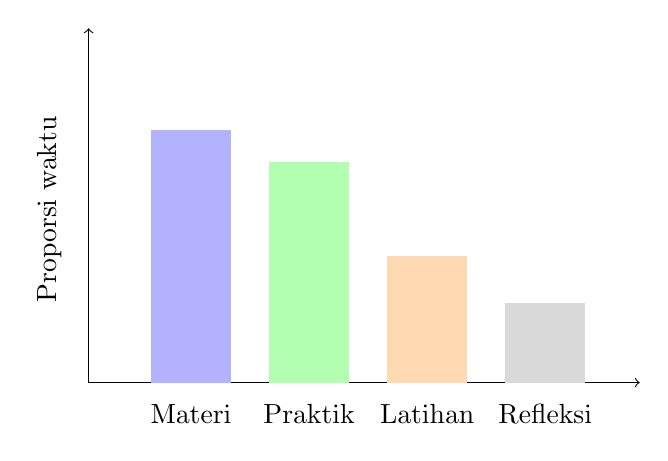
\begin{tikzpicture}
    \draw[->] (0,0) -- (0,4.5);
    \draw[->] (0,0) -- (7,0);
    \filldraw[blue!30] (0.8,0) rectangle (1.8,3.2);
    \filldraw[green!30] (2.3,0) rectangle (3.3,2.8);
    \filldraw[orange!30] (3.8,0) rectangle (4.8,1.6);
    \filldraw[gray!30] (5.3,0) rectangle (6.3,1.0);
    \node at (1.3,-0.4) {Materi};
    \node at (2.8,-0.4) {Praktik};
    \node at (4.3,-0.4) {Latihan};
    \node at (5.8,-0.4) {Refleksi};
    \node[rotate=90] at (-0.5,2.2) {Proporsi waktu};
  \end{tikzpicture}
  \caption{Ilustrasi proporsi waktu belajar per komponen (dapat disesuaikan).}
\end{figure}

\section{Ringkasan Konteks Kurikulum OBE}

Pendekatan \textit{Outcome-Based Education} (OBE) menggeser fokus pendidikan dari "apa yang diajarkan" menjadi "apa yang mampu dilakukan oleh mahasiswa" setelah proses pembelajaran selesai. Dalam sistem ini, keberhasilan pendidikan tidak diukur dari berapa banyak jam materi yang tersampaikan, melainkan dari bukti nyata capaian kompetensi yang dapat ditunjukkan oleh mahasiswa pada akhir periode belajar \cite{obe_wikipedia}.

Oleh karena itu, \textit{learning outcomes} dalam buku ini disusun menggunakan kata kerja operasional yang spesifik dan terukur agar dapat diamati serta diases secara objektif \cite{adelaide_learning_outcomes,stanford_learning_outcomes}. Dalam konteks mata kuliah Kriptografi, hirarki kurikulum yang diterapkan adalah sebagai berikut:

\begin{enumerate}
    \item \textbf{CPL (Capaian Pembelajaran Lulusan)}: Merupakan profil kompetensi akhir yang harus dimiliki oleh setiap lulusan Program Studi Teknik Informatika. Ini adalah standar kualitas lulusan yang mencakup aspek sikap, pengetahuan, dan keterampilan.
    \item \textbf{CPMK (Capaian Pembelajaran Mata Kuliah)}: Merupakan turunan dari CPL yang menjadi target utama mata kuliah Kriptografi. Contohnya adalah kemampuan \textit{mengenal} algoritma kriptografi (CPMK-1) dan \textit{memahami} urgensi keamanan informasi (CPMK-2).
    \item \textbf{Sub-CPMK}: Merupakan indikator pencapaian yang lebih detail dan spesifik. Sub-CPMK inilah yang menjadi acuan dalam penyusunan setiap bab, aktivitas praktikum, soal latihan, dan instrumen asesmen di dalam buku ini.
\end{enumerate}

Implementasi OBE dalam buku ini menuntut adanya keterhubungan yang kuat antara aktivitas pembelajaran dan indikator capaian. Buku ini menekankan penggunaan \textbf{asesmen formatif} (latihan dan aktivitas di tengah bab) serta \textbf{refleksi diri} (checklist kompetensi), sehingga mahasiswa dapat memantau kemajuan belajarnya secara mandiri, mengenali kesenjangan kompetensi yang masih ada, dan mengambil langkah perbaikan secara proaktif sebelum menghadapi asesmen sumatif (ujian).

\section{Ikhtisar Materi per Bab}

Struktur kurikulum kriptografi ini dirancang secara sistematis untuk membangun pemahaman dari konsep dasar hingga aplikasi lanjutan. Setiap bab mengintegrasikan teori matematis, implementasi praktis, dan analisis keamanan untuk memberikan pembelajaran yang komprehensif dan berorientasi aplikasi.

\begin{enumerate}
  \item \textbf{Bab II}: Pengantar kriptografi, model keamanan, ancaman, confidentiality, integrity, authenticity, kriptografi simetris vs asimetris
  \item \textbf{Bab III}: Aritmetika modular, algoritma Euclid, teori bilangan, fast exponentiation, implementasi C
  \item \textbf{Bab IV}: Cipher Caesar, substitusi monoalfabetik, Vigenère, kelemahan cipher klasik, implementasi C
  \item \textbf{Bab V}: Block cipher, DES, AES, mode operasi ECB, CBC, CFB, OFB
  \item \textbf{Bab VI}: Kriptografi asimetris, RSA, pembangkitan kunci, enkripsi/dekripsi, implementasi C
  \item \textbf{Bab VII}: Fungsi hash (SHA, MD5), integritas data, tanda tangan digital
  \item \textbf{Bab VIII}: Protokol Diffie-Hellman, TLS dasar, manajemen kunci
  \item \textbf{Bab IX}: Kriptanalisis, frequency analysis, Kasiski examination
  \item \textbf{Bab X}: Evaluasi komprehensif dan rubrik penilaian. Tinjauan pencapaian serta rekomendasi tindak lanjut.
\end{enumerate}

Perjalanan pembelajaran dimulai dengan fondasi teoretis yang kuat pada Bab II dan III, memberikan pemahaman tentang prinsip-prinsip dasar keamanan informasi dan alat matematika yang diperlukan. Bab IV dan V memperkenalkan implementasi praktis mulai dari cipher klasik hingga block cipher modern, membangun keterampilan pemrograman dan analisis secara bertahap. Pendekatan ini memastikan mahasiswa memiliki dasar yang kokoh sebelum beralih ke konsep yang lebih kompleks.

Bab VI hingga VIII membahas teknologi kriptografi modern yang secara luas digunakan dalam industri, termasuk RSA, fungsi hash, dan protokol pertukaran kunci. Materi-materi ini dirancang untuk menghubungkan konsep akademis dengan aplikasi dunia nyata yang ditemui dalam sistem keamanan digital. Bab IX menambahkan perspektif keamanan dengan mempelajari teknik kriptanalisis, memberikan pemahaman holistik tentang kekuatan dan kelemahan sistem enkripsi.

Bab penutup (X) mengintegrasikan semua pengetahuan yang telah dipelajari melalui evaluasi komprehensif dan refleksi diri. Bab ini dirancang untuk mengukur pencapaian kompetensi secara keseluruhan dan memberikan rekomendasi pengembangan lebih lanjut bagi mahasiswa. Struktur kurikulum ini memastikan lulusan memiliki pemahaman mendalam tentang kriptografi dari perspektif teoretis, praktis, dan keamanan, mempersiapkan mereka untuk karir di bidang keamanan siber.


% ============================================================
% Rangkuman Bab
% ============================================================
\begin{rangkuman}
Bab ini memperkenalkan tujuan buku ajar, keterkaitan dengan RPS berbasis OBE, petunjuk penggunaan, dan konteks kurikulum OBE. Pemahaman yang baik tentang struktur dan pendekatan buku ini akan membantu Anda memaksimalkan pembelajaran Kriptografi.

\textbf{Poin Kunci:}
\begin{itemize}
  \item Buku ini dirancang dengan pendekatan OBE yang fokus pada pencapaian kompetensi terukur
  \item Setiap bab dipetakan ke Sub-CPMK yang berkontribusi pada CPL
  \item Gunakan komponen OBE (Sub-CPMK, aktivitas, latihan, asesmen, checklist) secara optimal
  \item Pembelajaran kriptografi tersusun sistematis dari landasan teori hingga implementasi C
\end{itemize}
\end{rangkuman}

% ============================================================
% Persiapan untuk Bab Berikutnya
% ============================================================
\begin{transition}
Setelah memahami struktur dan pendekatan pembelajaran dalam buku ini, kita akan memasuki \textbf{Bab II: Landasan Teori dan Konsep Dasar Kriptografi}. 

Dalam Bab II, Anda akan:
\begin{itemize}
  \item Memahami \textit{big picture} keamanan informasi: mengapa kriptografi diperlukan
  \item Mengenal terminologi dasar: plaintext, ciphertext, cipher, key
  \item Memahami layanan keamanan: confidentiality, integrity, availability,\\ non-repudiation
  \item Mengenali model komunikasi aman dan ancaman yang ada
  \item Membedakan kriptografi simetris dan asimetris
\end{itemize}

Pemahaman konsep dasar ini akan menjadi fondasi yang penting sebelum kita mempelajari matematika kriptografi di Bab III. Setiap konsep yang dipelajari di Bab II akan terus kita rujuk dan kembangkan dalam bab-bab berikutnya.
\end{transition}

\ifSubfilesClassLoaded{
  \renewcommand{\bibname}{Daftar Pustaka}
  \bibliographystyle{plain}
  \bibliography{../references}
}{}
\end{document}
